\evenchapter[Définition du sujet]{Définition du sujet}

\textit{Le présent chapitre a pour objectif de ... . }

\section{Contextualisation du sujet}

Grâce au développement des techniques LiDAR et aux prises de vues aériennes et satellites, il est aujourd’hui facile de représenter des objets en volume. Cette modélisation peut passer par la création d’un nuage de points, mais également par les Modèles Numériques de Surface (MNS) pour les applications topographiques. Ces MNS permettent de représenter le terrain, mais aussi les constructions, la végétation, les voies de circulation, … .\newline

\begin{wrapfigure}[18]{r}{7cm}
	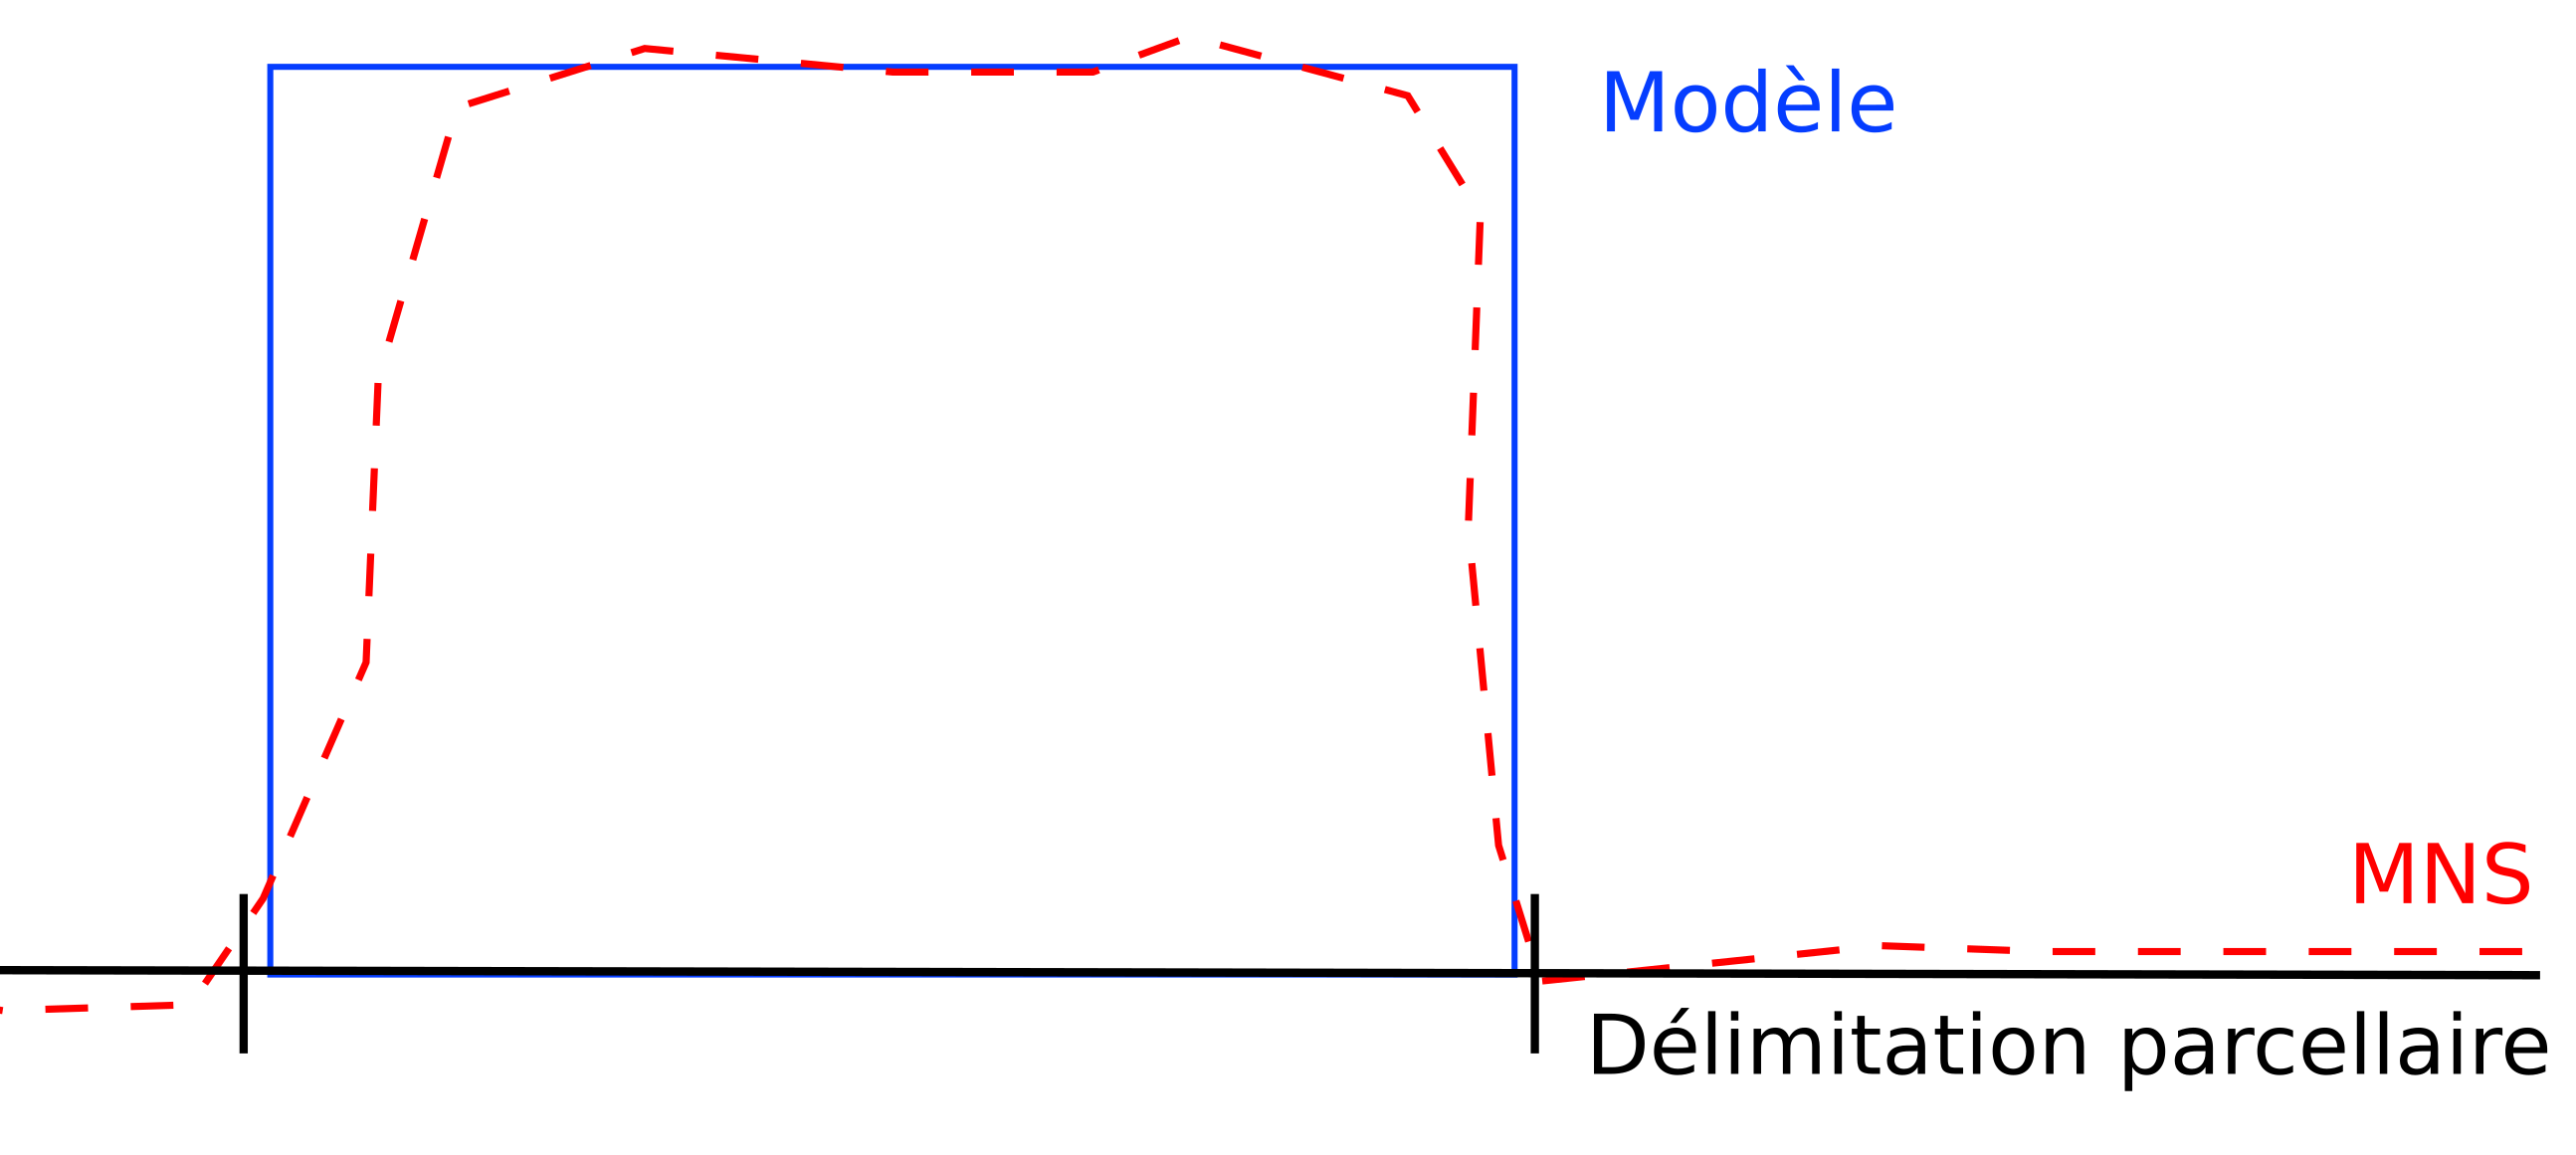
\includegraphics[width=6.5cm]{Correlation_modele3D_terrain(1).png}
	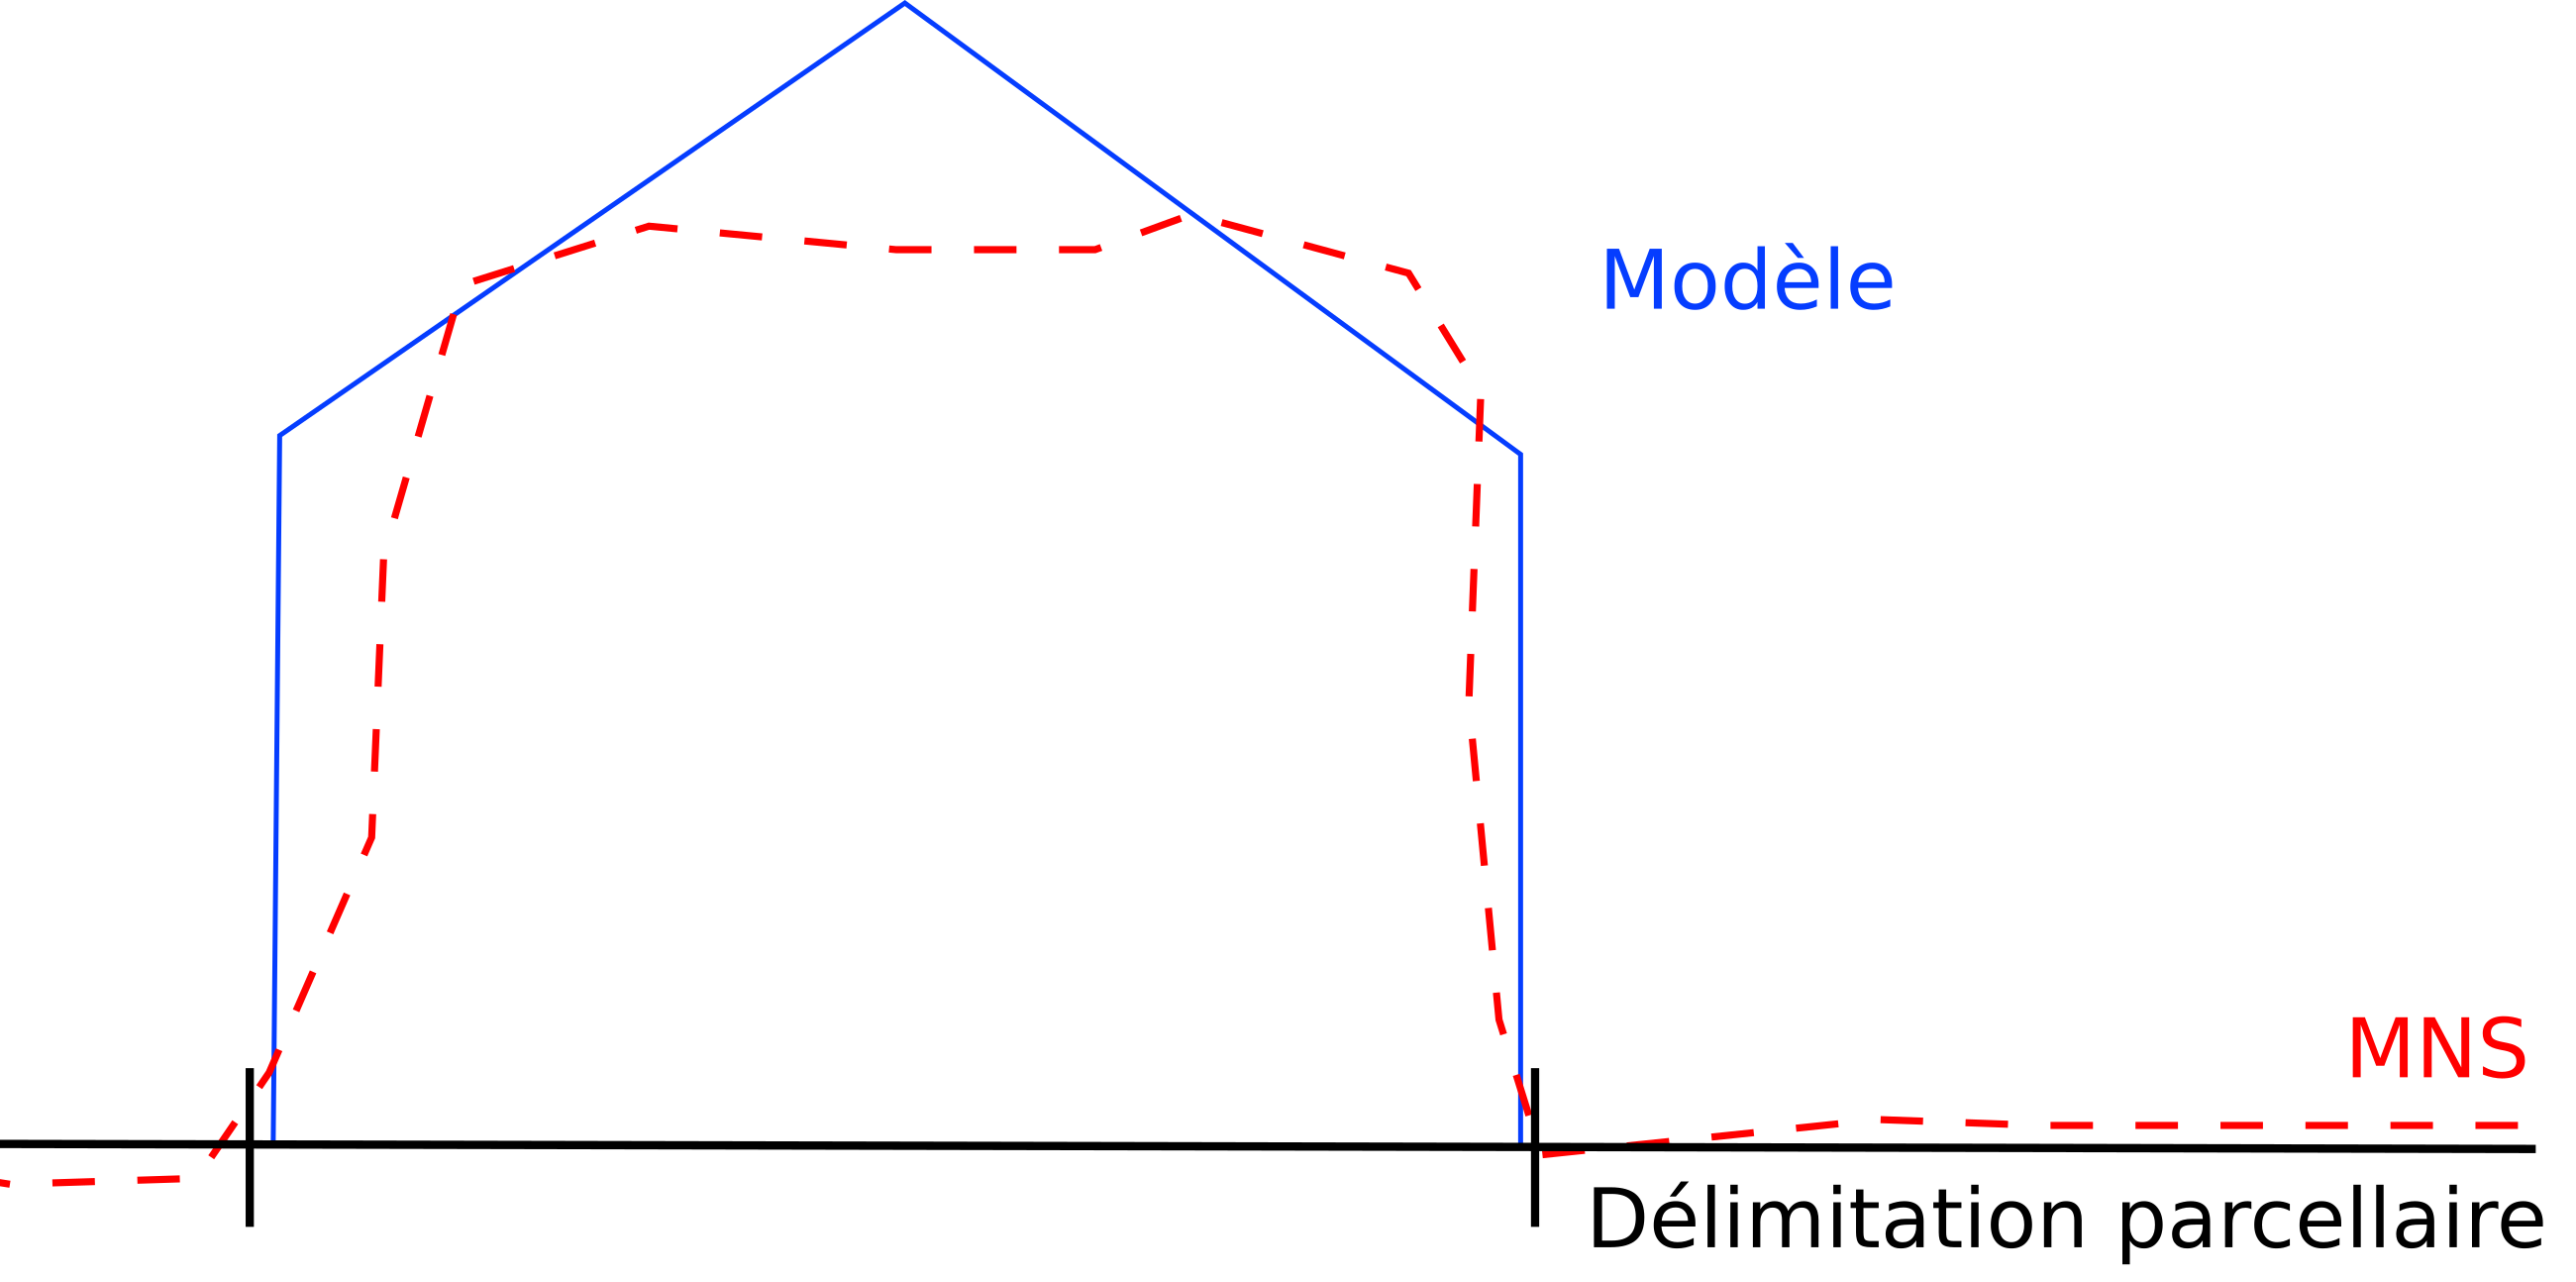
\includegraphics[width=6.5cm]{Correlation_modele3D_terrain(2).png}
	\caption{Association d'un modèle 3D au terrain}
	\label{Association d'un modèle 3D au terrain}
\end{wrapfigure}
Le projet présenté s’inscrit dans le cadre des recherches du MATIS pour la reconstruction 3D des bâtiments à partir de MNS. Pour ce faire, on cherche à associer un modèle prédéfini de bâtiment 3D à un objet numérique, reconstitué par le MNS et l’emprise au sol du bâtiment. Cette phase d’association est basée sur les principes de corrélation d’objet. \newline

Suivant le niveau de détail recherché, différents modèles sont possibles : Manhattan (= toits plats), Biplan (= toits pentus), Modélisation précise (à partir de la triangulation du MNS), … Plus le modèle est évolué, plus le niveau de détail est important mais plus la généralisation est compliquée et lourde à coder.\newline

\begin{figure}[!h]
	\begin{center}
		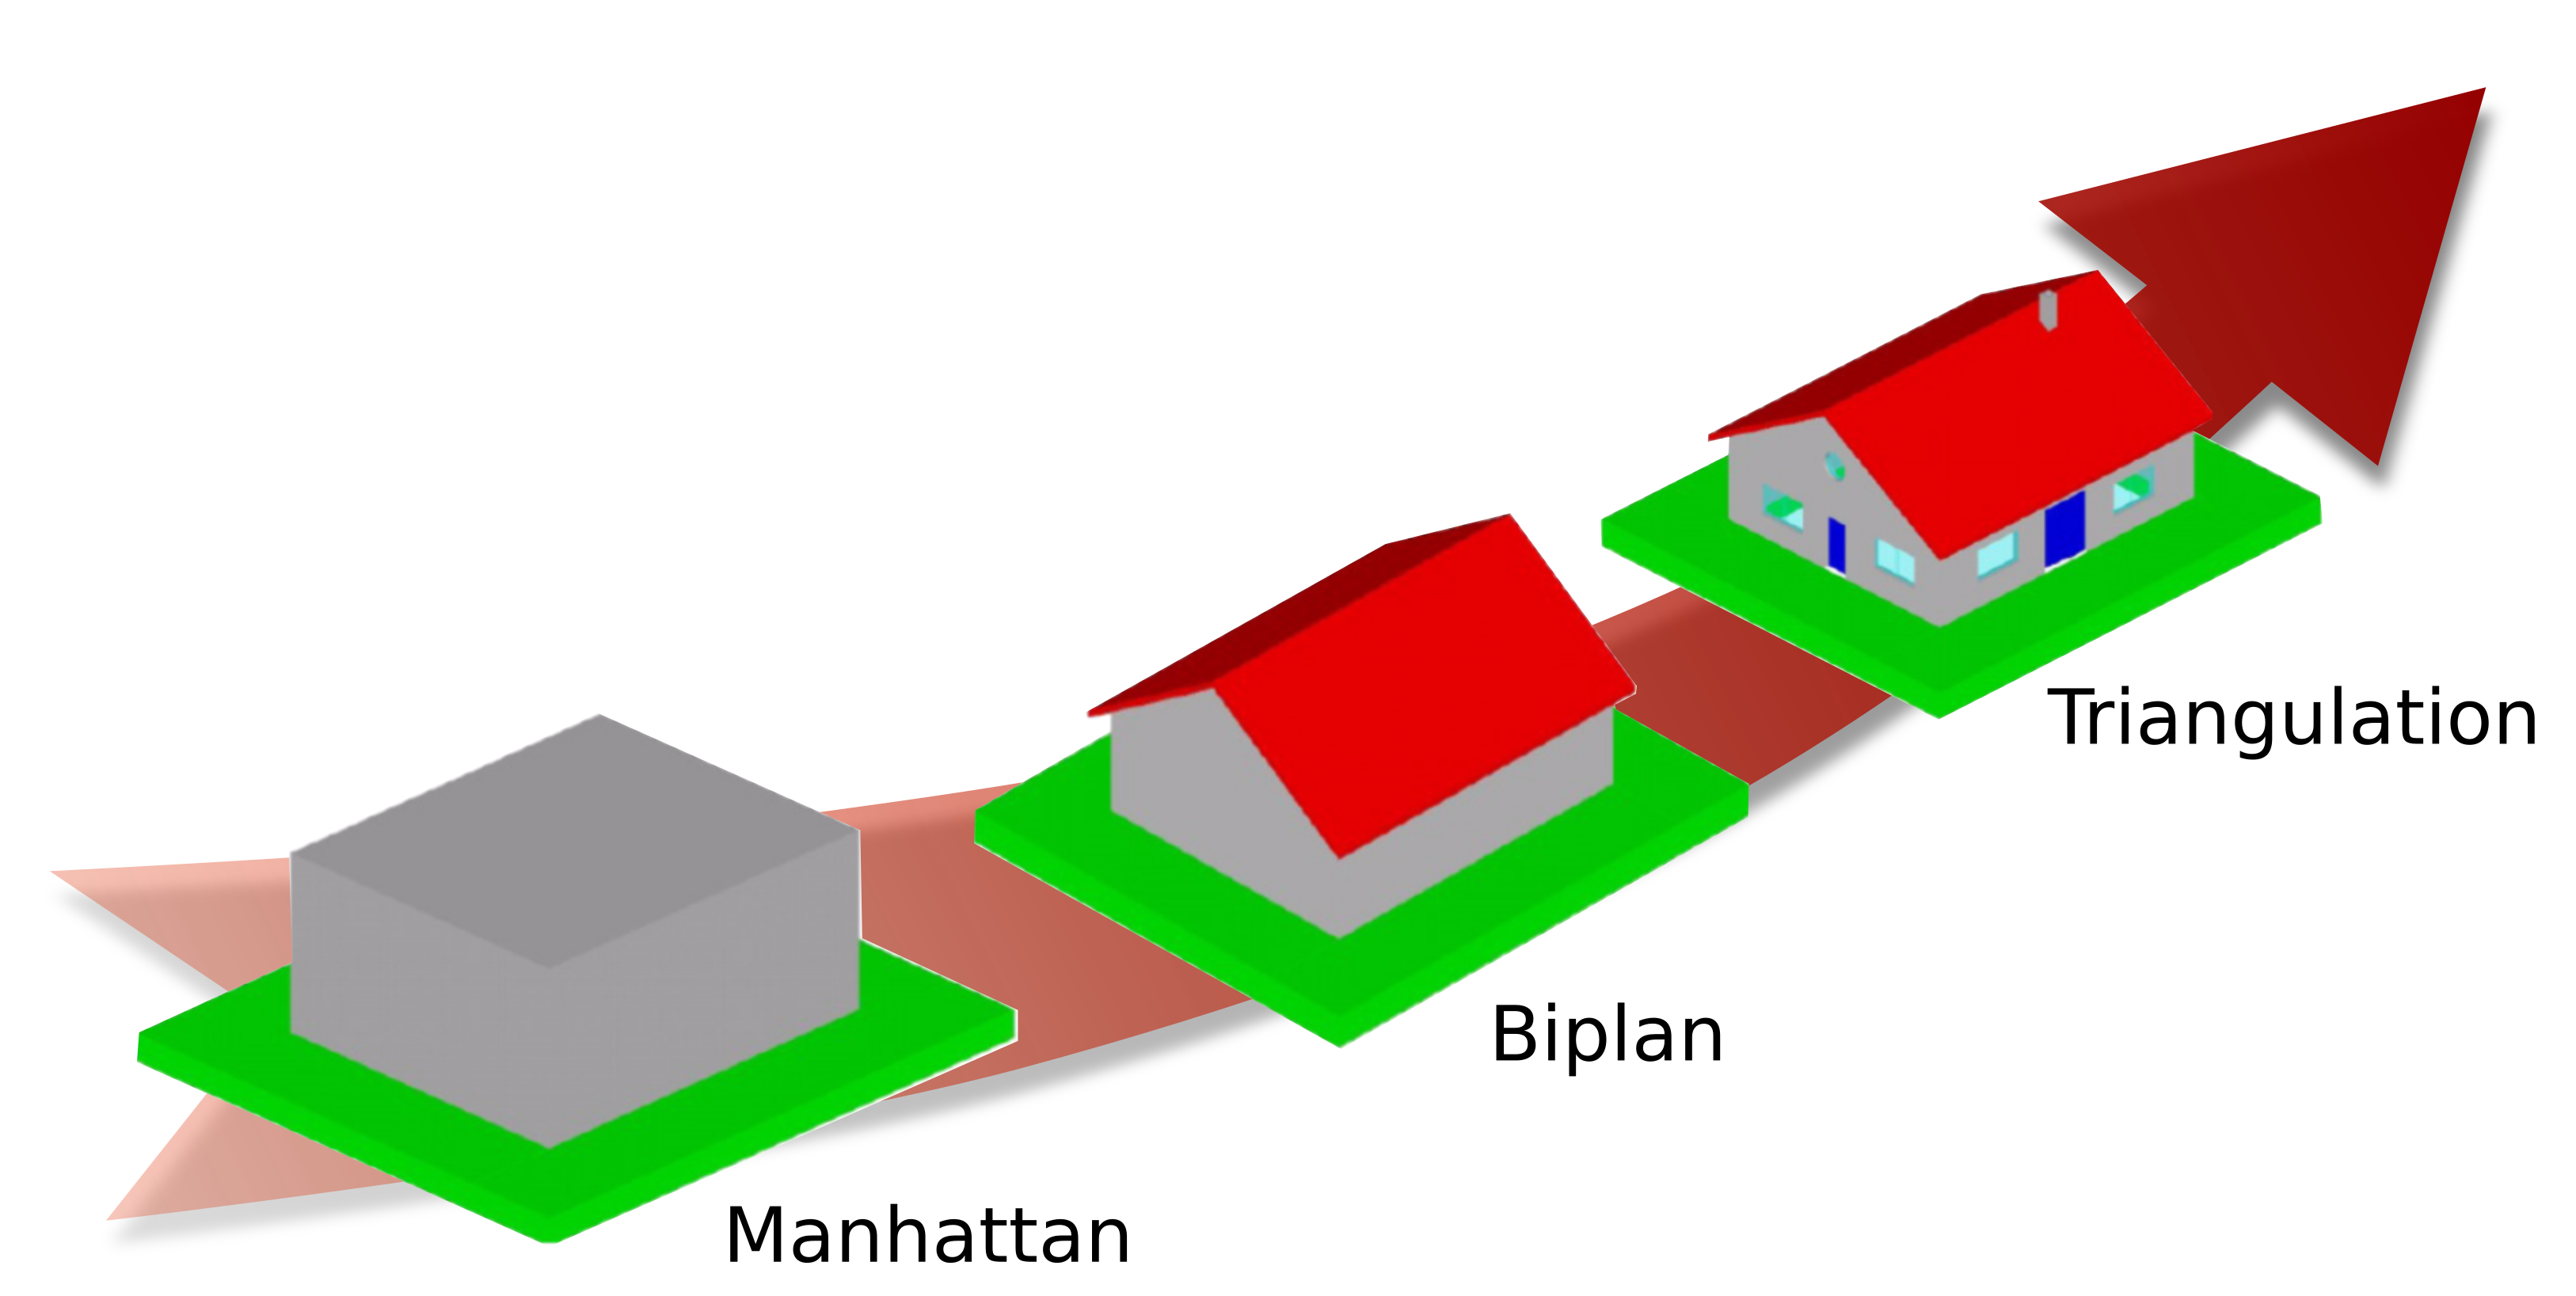
\includegraphics[scale=0.13]{Niveau_detail.png}  \\
		\caption[Niveau de détail des modèles 3D]{Niveau de détail des modèles 3D}
		\label{fig:example}
	\end{center}
\end{figure}

\newpage Cependant, aucune méthode de reconstruction n’est totalement fiable. Pour détecter et caractériser ces erreurs, l’équipe de recherche à mis en place une méthode automatique de classification des entités (sous-découpage des parcelles, erreur de pentes du toit, mauvaise forme, …). Dans certains cas, il est encore difficile d’estimer les bonnes classes d’intérêt, et un utilisateur pourrait permettre de valider ou non les résultats de la classification. \newline 

\section{Problématique}

Le projet consiste à réaliser une interface pour interagir avec un utilisateur dans le cadre de l'amélioration des classifications. 
